\documentclass[ngerman,a4paper,11pt,twoside,cleardoubleempty,halfparskip]{scrreprt}

% Erforderliche Pakete
\usepackage[utf8]{inputenc}
\usepackage{babel}
\usepackage{graphicx}
\usepackage{fancyhdr}
\usepackage{multirow}
\usepackage{ifthen}
\usepackage{calc}
\usepackage{tabularx}
\usepackage{listings}
\usepackage[autokw]{svn-multi}
\usepackage[toc]{glossaries}
\usepackage[implicit=false]{hyperref} % implizit stört irgendwie beim Lesen

% weiteren, nützliche Pakete
%\usepackage{subfigure} 
%\usepackage{varioref}
%\usepackage{framed}
%\usepackage{longtable}
%\usepackage{floatflt}
%\usepackage{amsmath}
%\usepackage{url}
% ...

% Pakete für Verzeichnisse. Diese sind hier aufgeführt, da mindestens das
% 'glossaries' Paket nach z.B. hyperref geladen werden muss.
\usepackage{bibgerm}

\svnid{$Id: design.tex 180 2012-05-24 15:26:04Z dgens001 $}

% Glossar(e) laden und erstellen
\makeglossaries
\loadglsentries{meta/glossar} % Name der Glossardatei (ohne .tex)

% Befehlsdefinitionen
\newcommand{\clearemptydoublepage}{\newpage{\pagestyle{empty}\cleardoublepage}}

% Globale Formatierungseinstellungen
%\renewcommand*\cleardoublepage{\clearpage\if@twoside \ifodd\c@page
%  \hbox{}\newpage\if@twocolumn\hbox{}\newpage\fi\fi\fi}
\renewcommand{\encodingdefault}{OT1}
\renewcommand{\familydefault}{cmss} % Schriftfamilie auf Sans Serif
\renewcommand{\glsdisplayfirst}[4]{\textit{#1#4}}
\setcapindent{1em}

% Anpassung der Ränder und Breitenverhältnisse
% Der letzte Wert in oddsidemargin bestimmt die Bindekorrektur
\setlength{\oddsidemargin}{2cm - 1in + 0.5cm}
\setlength{\textwidth}{\paperwidth - (1in + \hoffset) - \oddsidemargin - 4cm}
\setlength{\evensidemargin}{\paperwidth - (1in + \hoffset)*2 - \oddsidemargin - \textwidth}
\setlength{\marginparwidth}{4cm - \marginparsep{} - 1cm}

% Wenn größerer Zeilenabstand gewünscht ist, je nach Schriftgröße:
% Abstand        10pt    11pt    12pt
% -----------------------------------
% anderthalb     1.25    1.21    1.24
% doppelt        1.67    1.62    1.66
%
%\renewcommand{\baselinestretch}{1.21}

% Kopf- und Fußzeilen einrichten
\pagestyle{plain}
\setlength{\headwidth}{\textwidth}
\addtolength{\headwidth}{\marginparsep}
\addtolength{\headwidth}{\marginparwidth}
\renewcommand{\chaptermark}[1]{\markboth{#1}{}}
\renewcommand{\sectionmark}[1]{\markright{\thesection\ #1}}
\lhead[\fancyplain{}{\bfseries\thepage}]%
	{\fancyplain{}{\bfseries\rightmark}}
\rhead[\fancyplain{}{\bfseries\leftmark}]%
	{\fancyplain{}{\bfseries\thepage}}
\cfoot{}

\begin{document}
\pagenumbering{arabic}
\svnid{$Id: titel.tex 180 2012-05-24 15:26:04Z dgens001 $}
\begin{titlepage}
	\begin{center}
		% Kopf der Seite
		
\includegraphics{meta/hsrm-logo} \\[0.7cm]
		{Fachbereich Design Informatik Medien}
		
		\vfill

		% Titel
		%\rule{\textwidth}{1pt}\\[0.5cm]
		{\huge \bfseries Designspezifikation Campusadventure}\\[0.1cm]
                im Fach Softwaretechnik im SS2012
		%\rule{\textwidth}{1pt}
		
		\vfill
		% Mitte der Seite
		\begin{tabular}{lr}
			Vorgelegt von & \line(1,0){100} \\
						  & Dominik Schuhmann \\ 
						  & \\
						  & \line(1,0){100} \\
                          & Tino Landmann \\ 
						  & \\
						  & \line(1,0){100} \\
                          & Simon Hardt \\
						  & \\
						  & \line(1,0){100} \\
                          & David Gens \\
                        \\
						\\
                        \\
						\\
			bei           & Prof. Dr. Wolfgang Weitz \\
                        \\
						am			  & \today \\
						\\
                        in der Version       &	\svnrev. \\
		\end{tabular}
		\vfill
		
		% Fuß der Seite
		
	\end{center}
\end{titlepage}
 % Titelseite (wird automatisch mit Werten von oben gefüllt)
\clearemptydoublepage % Sorgt dafür, dass die nächste Seite rechts beginnt

  \begin{longtable}{l l l p{80px} p{200px}}
	  \textbf{Rev} & \textbf{Autor}  &\textbf{Datum} & \textbf{Beschreibung} & \textbf{Dateien}\\
	  \hline
	              &      \           &       \       &            \          &        \\
	  181 &
		  tland001
		  &
		  24-05-2012
		  &
		  lautfzeitdiagram bla2
		  & \strut
		  /design/kapitel/laufzeitsicht.tex \par  \strut \\
	  180 &
		  dgens001
		  &
		  24-05-2012
		  &
		  svn tag mal gesetzt.. wäre clever gewesen
		  & \strut
		  /design/kapitel/bausteinsicht.tex \par /design/meta/svnlog.tex \par /design/kapitel/musterundkonzepte.tex \par /design/meta/glossar.tex \par /design/design.pdf \par /design/meta/titel.tex \par /design/kapitel/laufzeitsicht.tex \par /design/kapitel/einfuehrung.tex \par /design/design.tex \par /design/kapitel/entwurfsentscheidungen.tex \par  \strut \\
	  179 &
		  dgens001
		  &
		  24-05-2012
		  &
		  laufzeitdiagramme umbenannt und beispielhaft eingefuegt
		  & \strut
		  /design/kapitel/laufzeitsicht/Spiel Laden.png \par /design/kapitel/laufzeitsicht/spielLaden.png \par /design/kapitel/bausteinsicht.tex \par /design/meta/svnlog.tex \par /design/kapitel/laufzeitsicht/Spieler\_Steuerung.png \par /design/kapitel/musterundkonzepte.tex \par /design/design.pdf \par /design/kapitel/laufzeitsicht/Neues Spiel.png \par /design/kapitel/laufzeitsicht/neuesSpiel.png \par /design/kapitel/laufzeitsicht.tex \par /design/bewegen\_seq.vpp \par  \strut \\
	  
  \end{longtable}
   % die letzten paar SVN-Logs als TEX-Tabelle formatiert
                    % (siehe meta/svnlog-gen.sh und meta/svnlog.xslt)
\clearemptydoublepage
\tableofcontents % Inhaltsverzeichnis generieren
\clearemptydoublepage

% --------------------------------- Hauptteil ----------------------------------
% Im diesen Teil werden die einzelnen Kapitel eingefügt, die sinnvollerweise
% im Verzeichnis 'kapitel' abgelegt werden.
\svnid{$Id: einfuehrung.tex 180 2012-05-24 15:26:04Z dgens001 $}
\chapter{Einführung}
In folgendem Dokument werden die grundlegenden Designentscheidungen des Softwaretechnikprojektes 
definiert und spezifiziert. Die Anwendung wird in Java entwickelt.

Im Abschnitt 2 werden die verschiedenen Bausteine der Anwendung erklärt und näher beschrieben. 
Abschnitt 3 befasst sich dann mit deren Zusammenspiel - dargestellt anhand verschiedener Use-Cases. 
Die angewendeten Muster und Konzepte werden in Abschnitt 3 behandelt.

\svnid{$Id: bausteinsicht.tex 180 2012-05-24 15:26:04Z dgens001 $}
\chapter{Bausteinsicht}
\textit{In diesem Abschnitt soll die Struktur der Spiele-Software dargestellt werden.
Im Vordergrund stehen die Bausteine, deren Beziehungen und eine Übersicht darüber mit welchen
Klassen und Paketen die zuvor erarbeiteten Anforderungen umgesetzt werden. Die Übersicht wird
dabei schrittweise verfeinert.}



\section{Übersicht}
Das \gls{Spiel} ist grundlegend in drei Schichten eingeteilt, Darstellungs-, Logik- und 
Datenschicht. Die genauen Zusammenhänge werden im Folgenden erläutert und durch das unten stehende 
Schichten-Diagramm sowie die angehängte UML-"Tapete" verdeutlicht.


\
\\
\begin{figure}[h]
	\begin{center}
		%trim option's parameter order: left bottom right top , clip = true
		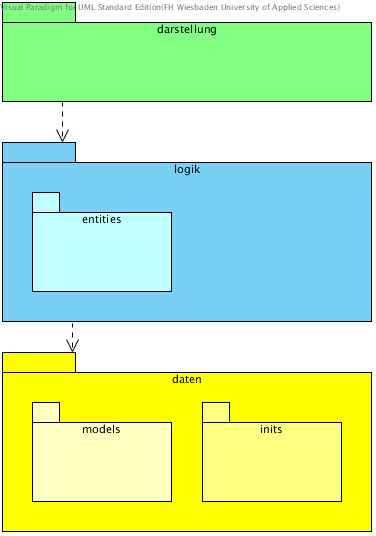
\includegraphics[height=7cm]{kapitel/bausteinsicht/schichten.png}
	\end{center}
	\caption{Architekturdiagramm}
	\label{fig:domain_uml}
\end{figure}



\section{Darstellung}
Die Darstellungsschicht beinhaltet verschiedene Klassen, die im Zusammenspiel letztlich die 
\gls{Anzeige} füllen. Die benötigte Kommunikation erfolgt dabei jeweils über 
\textit{PropertyChangeListener}, sodass Klassen der Logikschicht deren Pendants der 
Darstellungsschicht benachrichtigen können.

\
\\
\begin{figure}[h]
	\begin{center}
		%trim option's parameter order: left bottom right top , clip = true
		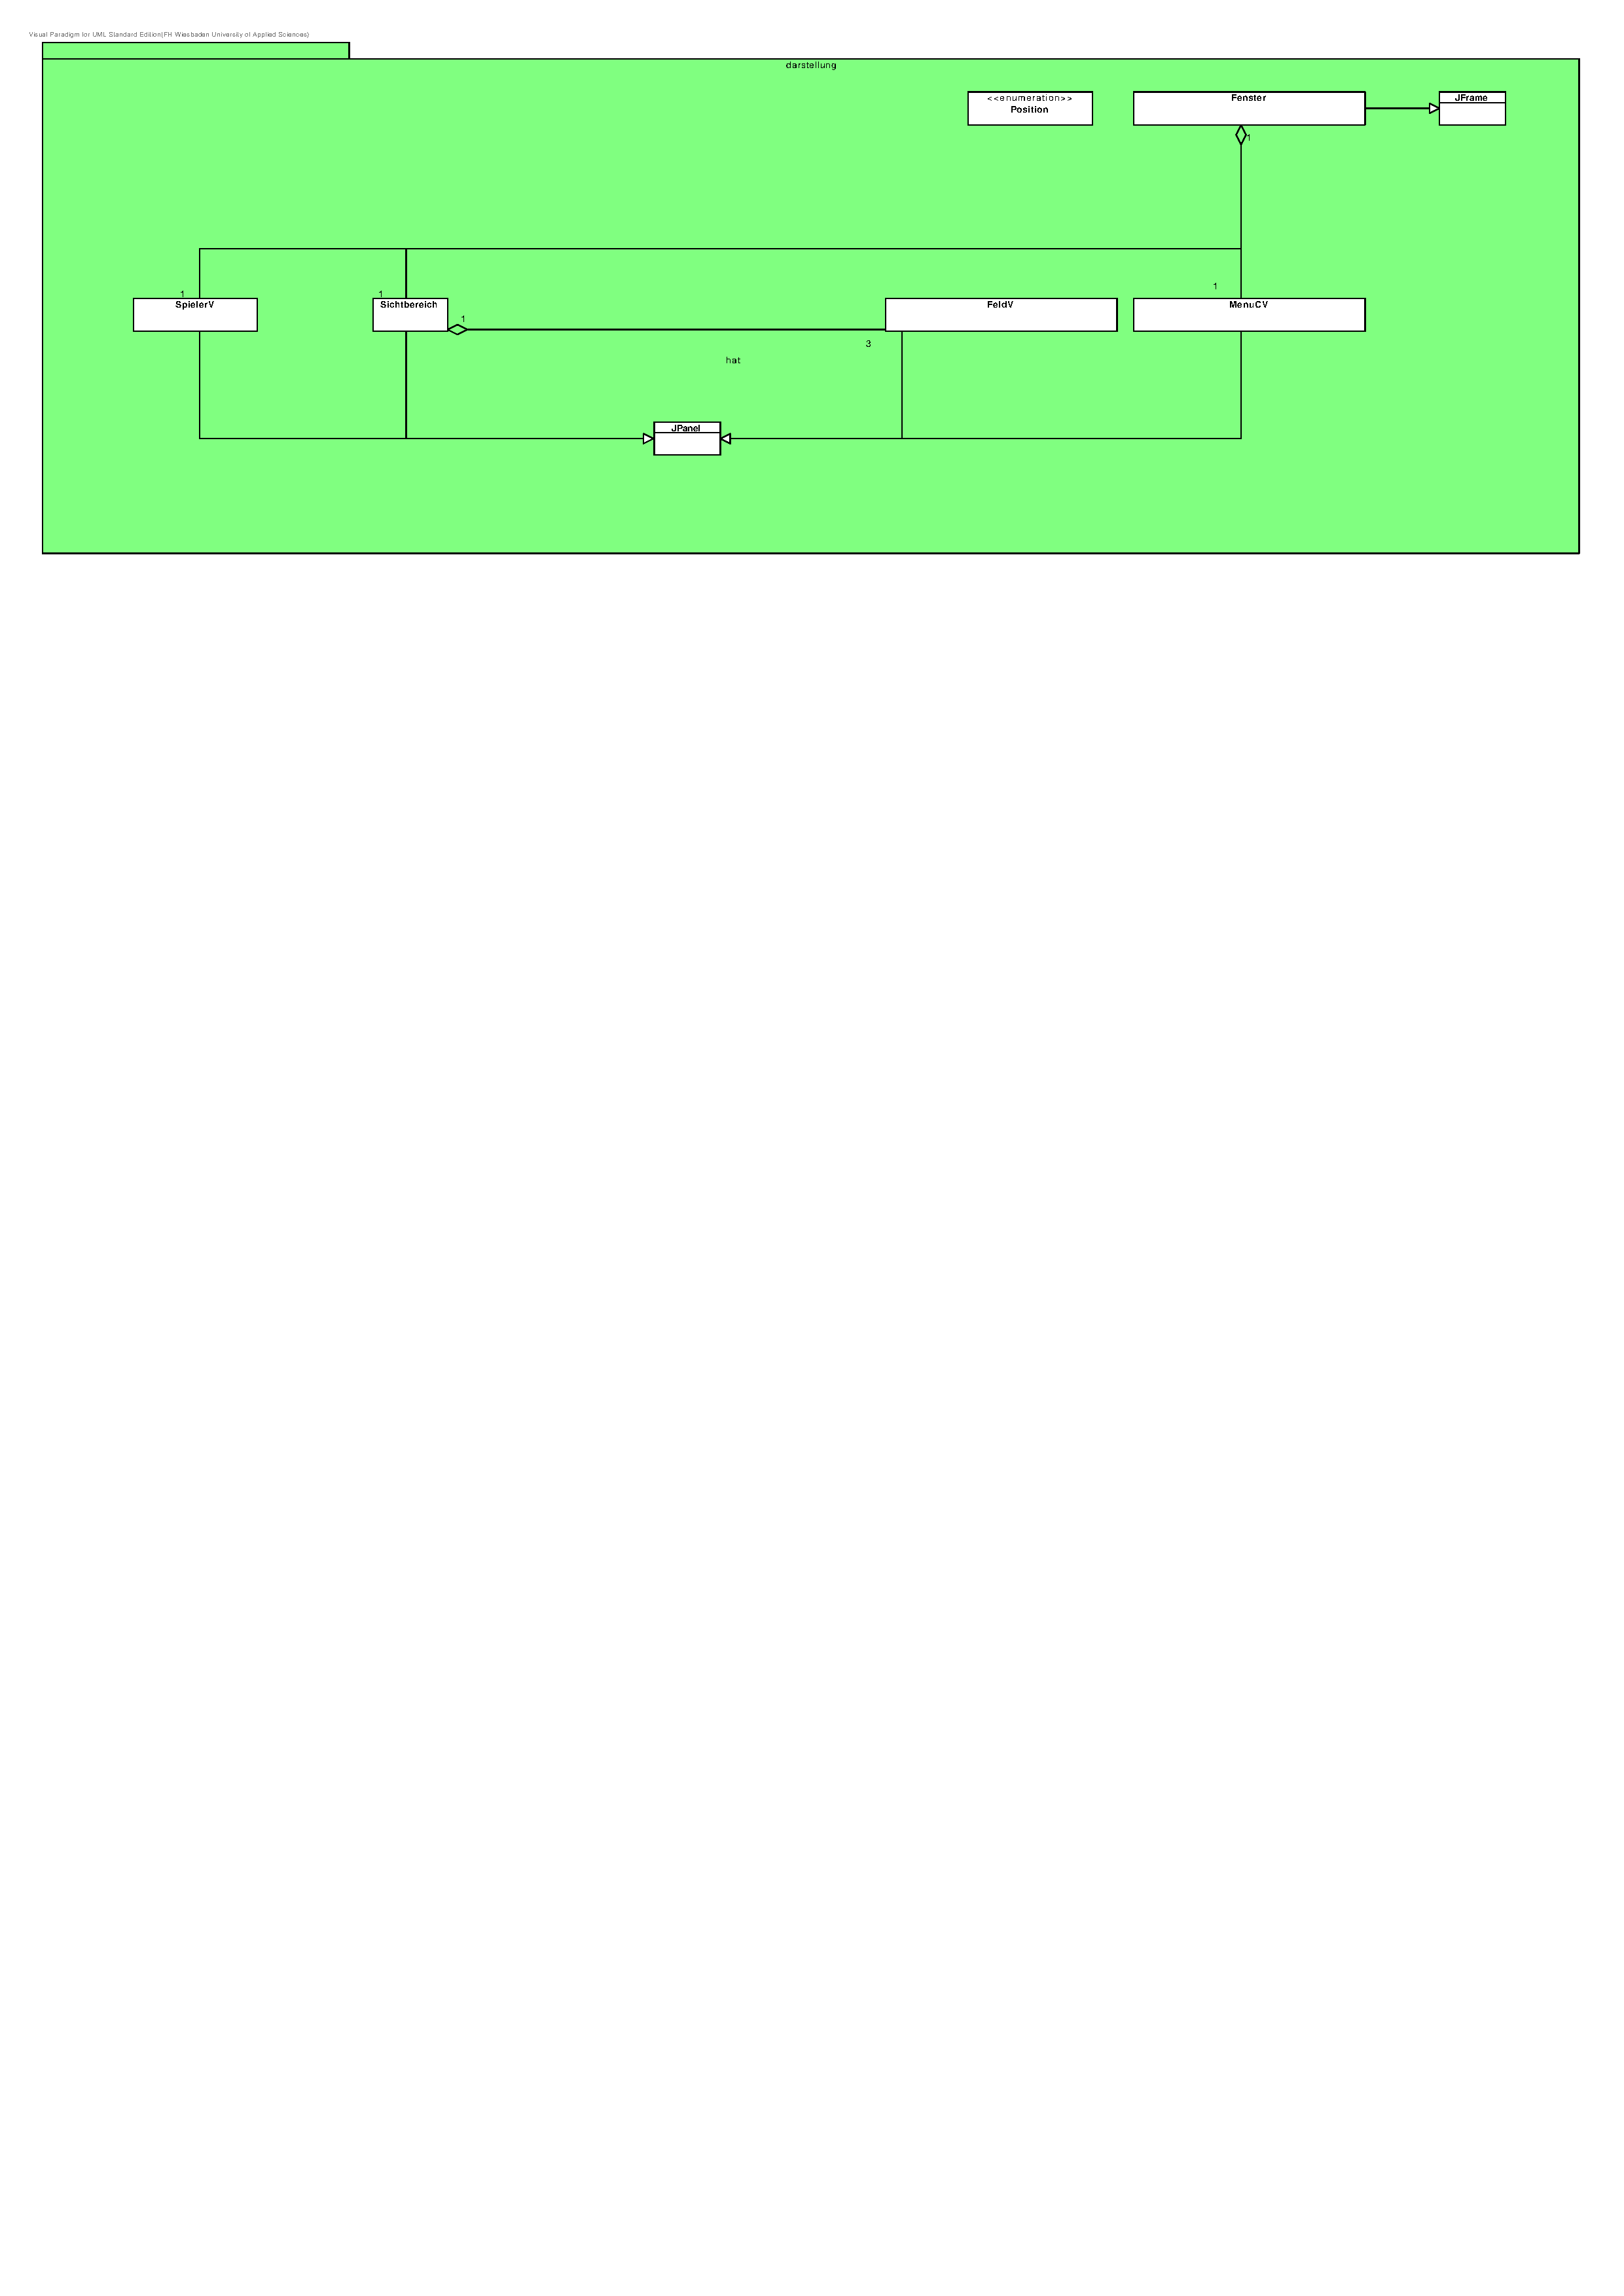
\includegraphics[trim=0cm 45cm 0cm 0cm, clip=true, width=16cm]{kapitel/bausteinsicht/darstellung.pdf}
	\end{center}
	\caption{Darstellungsschicht}
	\label{fig:darstellung_uml}
\end{figure}

\subsection{Fenster}
Das Fenster erweitert das Java \textit{JFrame} und zeigt die beiden Bereiche \gls{Statusbereich} 
(SpielerV) und \gls{Sichtbereich} (Szene) an. Falls sich der \gls{Spieler} in einem Menu befindet, 
zeigt das Fenster statt der beiden o.g. Bereiche nur das passende Menu (MenuCV) an.

\subsection{MenuCV}
Der \gls{Menuemodus} bietet dem \gls{Spieler} verschiedene Optionen an. Das Menu unterscheidet 
zudem selbst, welches Untermenu gezeigt wird. Dazu stehen z.B. die Funktionen \textit{drawPause()} 
oder \textit{drawSave()} bereit.

\subsection{Sichtbereich}
Der \gls{Sichtbereich} zeigt die \gls{Welt} in einer Pseudo-3D-Perspektive an. Es werden dabei immer 
die nächsten drei \glspl{Feld} in \gls{Blickrichtung} des \gls{Spieler}s mit ihren \glspl{GameObject} 
dargestellt. Die anderen Felder eines Raumes werden ohne evtl. \glspl{GameObject} gezeigt.

Die Darstellung der Felder mit \glspl{GameObject} erfolgt über drei \textit{FeldV}, welche die drei 
vorderen \glspl{Feld} in \gls{Blickrichtung} des \gls{Spieler}s darstellen. Diese werden von 
\textit{Sichtbereich} mit dem darzustellenden Feld und der benötigten Position des \gls{Feld}es 
(vorne, mitte, hinten).

Alle anderen \textit{JPanels} des \gls{Sichtbereich}s werden je nach Position des \gls{Spieler}s und 
dessen \gls{Blickrichtung} mit verschiedenen Texturen versehen, sodass ein räumlicher Eindruck entsteht.

\subsection{FeldV}
Die eigentliche Darstellung von \glspl{GameObject} auf den drei vorderen \glspl{Feld} wird von 
\textit{FeldV} übernommen, welches ein Raster anzeigt.

Dieses Raster zeigt die einzelnen \gls{Item}-, \gls{npc}- und \gls{Eingang}sanordnungen des 
\gls{Feld}es. Dazu wird die \textit{getObjects}-Methode der \gls{Feld}-Klasse vom View aufgerufen. 
Rückgabe ist hierbei eine Liste von \glspl{GameObject}, von welchen mit \textit{getImg()} deren 
Bild und evtl. Name angezeigt werden kann.

\subsection{SpielerV}
Der \textit{SpielerV} zeigt die Statusleiste an. Diese wird je nach Bedarf mit den passenden Inhalten 
gefüllt. Es wird z.B. das \gls{Inventar} und der Avatar des \gls{Spieler}s gezeigt. Tritt der 
\gls{Spieler} in Interaktion mit einem \gls{GameObject}, wird auch dazu der passende View gewählt. 
Die Auswahl erfolgt mit Hilfe der Funktionen \textit{drawInventar()}, \textit{drawInteraktion()}, 
\textit{drawHand()} und \textit{drawAvatar()}. Was zu tun ist, wird von \textit{Spieler} durch ein 
\textit{PropertyChangeEvent} angestoßen.

\paragraph{Infobereich}
Im \gls{Infobereich} werden je nach Situation das \gls{Inventar} des \gls{Spieler}s mit dessen Slots 
und den darin befindlichen \glspl{Gegenstand}n gezeigt oder textuelle Information bei Interaktionen 
dargestellt.

\paragraph{Handbereich}
Wählt der \gls{Spieler} die Interaktion mit einem \gls{Gegenstand} wird im \gls{Handbereich} das 
Bild des jeweiligen \gls{Item}s angezeigt. Im Normalfall wird eine leere Hand gezeigt.

\paragraph{Statusbereich}
Im \gls{Statusbereich} kann der \gls{Spieler} verschiedene Informationen zu sich selbst oder einem 
\gls{npc} erhalten. Meist wird ein Portät des jeweiligen Charakters dargestellt.

\subsubsection{Interaktion}
Die Methode \textit{drawInteraktion()} unterscheidet zudem den Typ des gewählten \gls{GameObject}s 
und füllt \gls{Infobereich}, \gls{Statusbereich} und \gls{Handbereich} mit den nötigen Inhalten. 

\paragraph{Interaktion mit Gegenständen}
% interaktion mit objekt
Bei der Interaktion mit einem \gls{Gegenstand} wird dessen Beschreibung und die möglichen 
Interaktionen, die der \gls{Spieler} damit tätigen kann, angezeigt. Er kann diese beispielsweise 
in sein \gls{Inventar} aufnehmen. Nimmt der \gls{Spieler} einen \gls{Gegenstand} auf, wird er zuerst 
in der Hand "zwischengespeichert". Das Bild des \gls{Gegenstand}s wird daher im \gls{Handbereich} 
angezeigt.

\paragraph{Interaktion mit NPCs}
Spricht der \gls{Spieler} hingegen einen \gls{npc} an, werden im \gls{Statusbereich} dessen Bild und 
Name gezeigt. Anhand des \textit{\gls{Dialog}Model}, stellt \textit{SpielerV} den \gls{Dialog} mit 
Text, Antworten und evtl. einem \gls{Item} dar, welches der \gls{Spieler} durch den letzten 
\gls{Dialog} erhalten hat.

\subsubsection{Inventar}
Der \gls{Spieler} besitzt ein \gls{Inventar} mit 10 Slots und eine \textit{Hand}. Diese kann 
lediglich einen einzigen \gls{Gegenstand} aufnehmen und dient als "Zwischenspeicher" bei einer 
Interaktion. Dargestellt werden \gls{Inventar} und Hand jeweils von \textit{drawInventar()} und 
\textit{drawHand()} der Klasse \textit{SpielerV}. Über den \glspl{Gegenstand}n im \gls{Inventar} 
werden Nummern angezeigt, die auf den passenden Index verweisen. Drückt der \gls{Spieler} eine 
dieser Nummern, wird der \gls{Gegenstand} aus dem \gls{Inventar} in die Hand genommen und beide 
Bereiche neu gezeichnet.
\newpage


\section{Logik}
In der Logik-Schicht befinden sich das Paket \textit{entities} und die Controller \textit{TastaturC} 
und \textit{GameC}.

Die hierin befindlichen Klassen sind jeweils möglichst autark - jegliche Funktionen, Interaktionen 
oder mögliches Zusammenspiel zwischen den Klassen/Objekten geschieht ohne Zutun einer dritten 
Instanz.

Ein Beispiel: Möchte der \gls{Spieler} einen \gls{Gegenstand} aufnehmen, wird die gesamte Logik vom 
\gls{Spieler} selbst übernommen - es gibt keine extra Klasse, die sich um den Ablauf kümmert. Zur 
Kommunikation zwischen den Klassen wird das Interface \textit{interagiere} verwendet.

\begin{figure}[h]
	\begin{center}
		%trim option's parameter order: left bottom right top , clip = true
		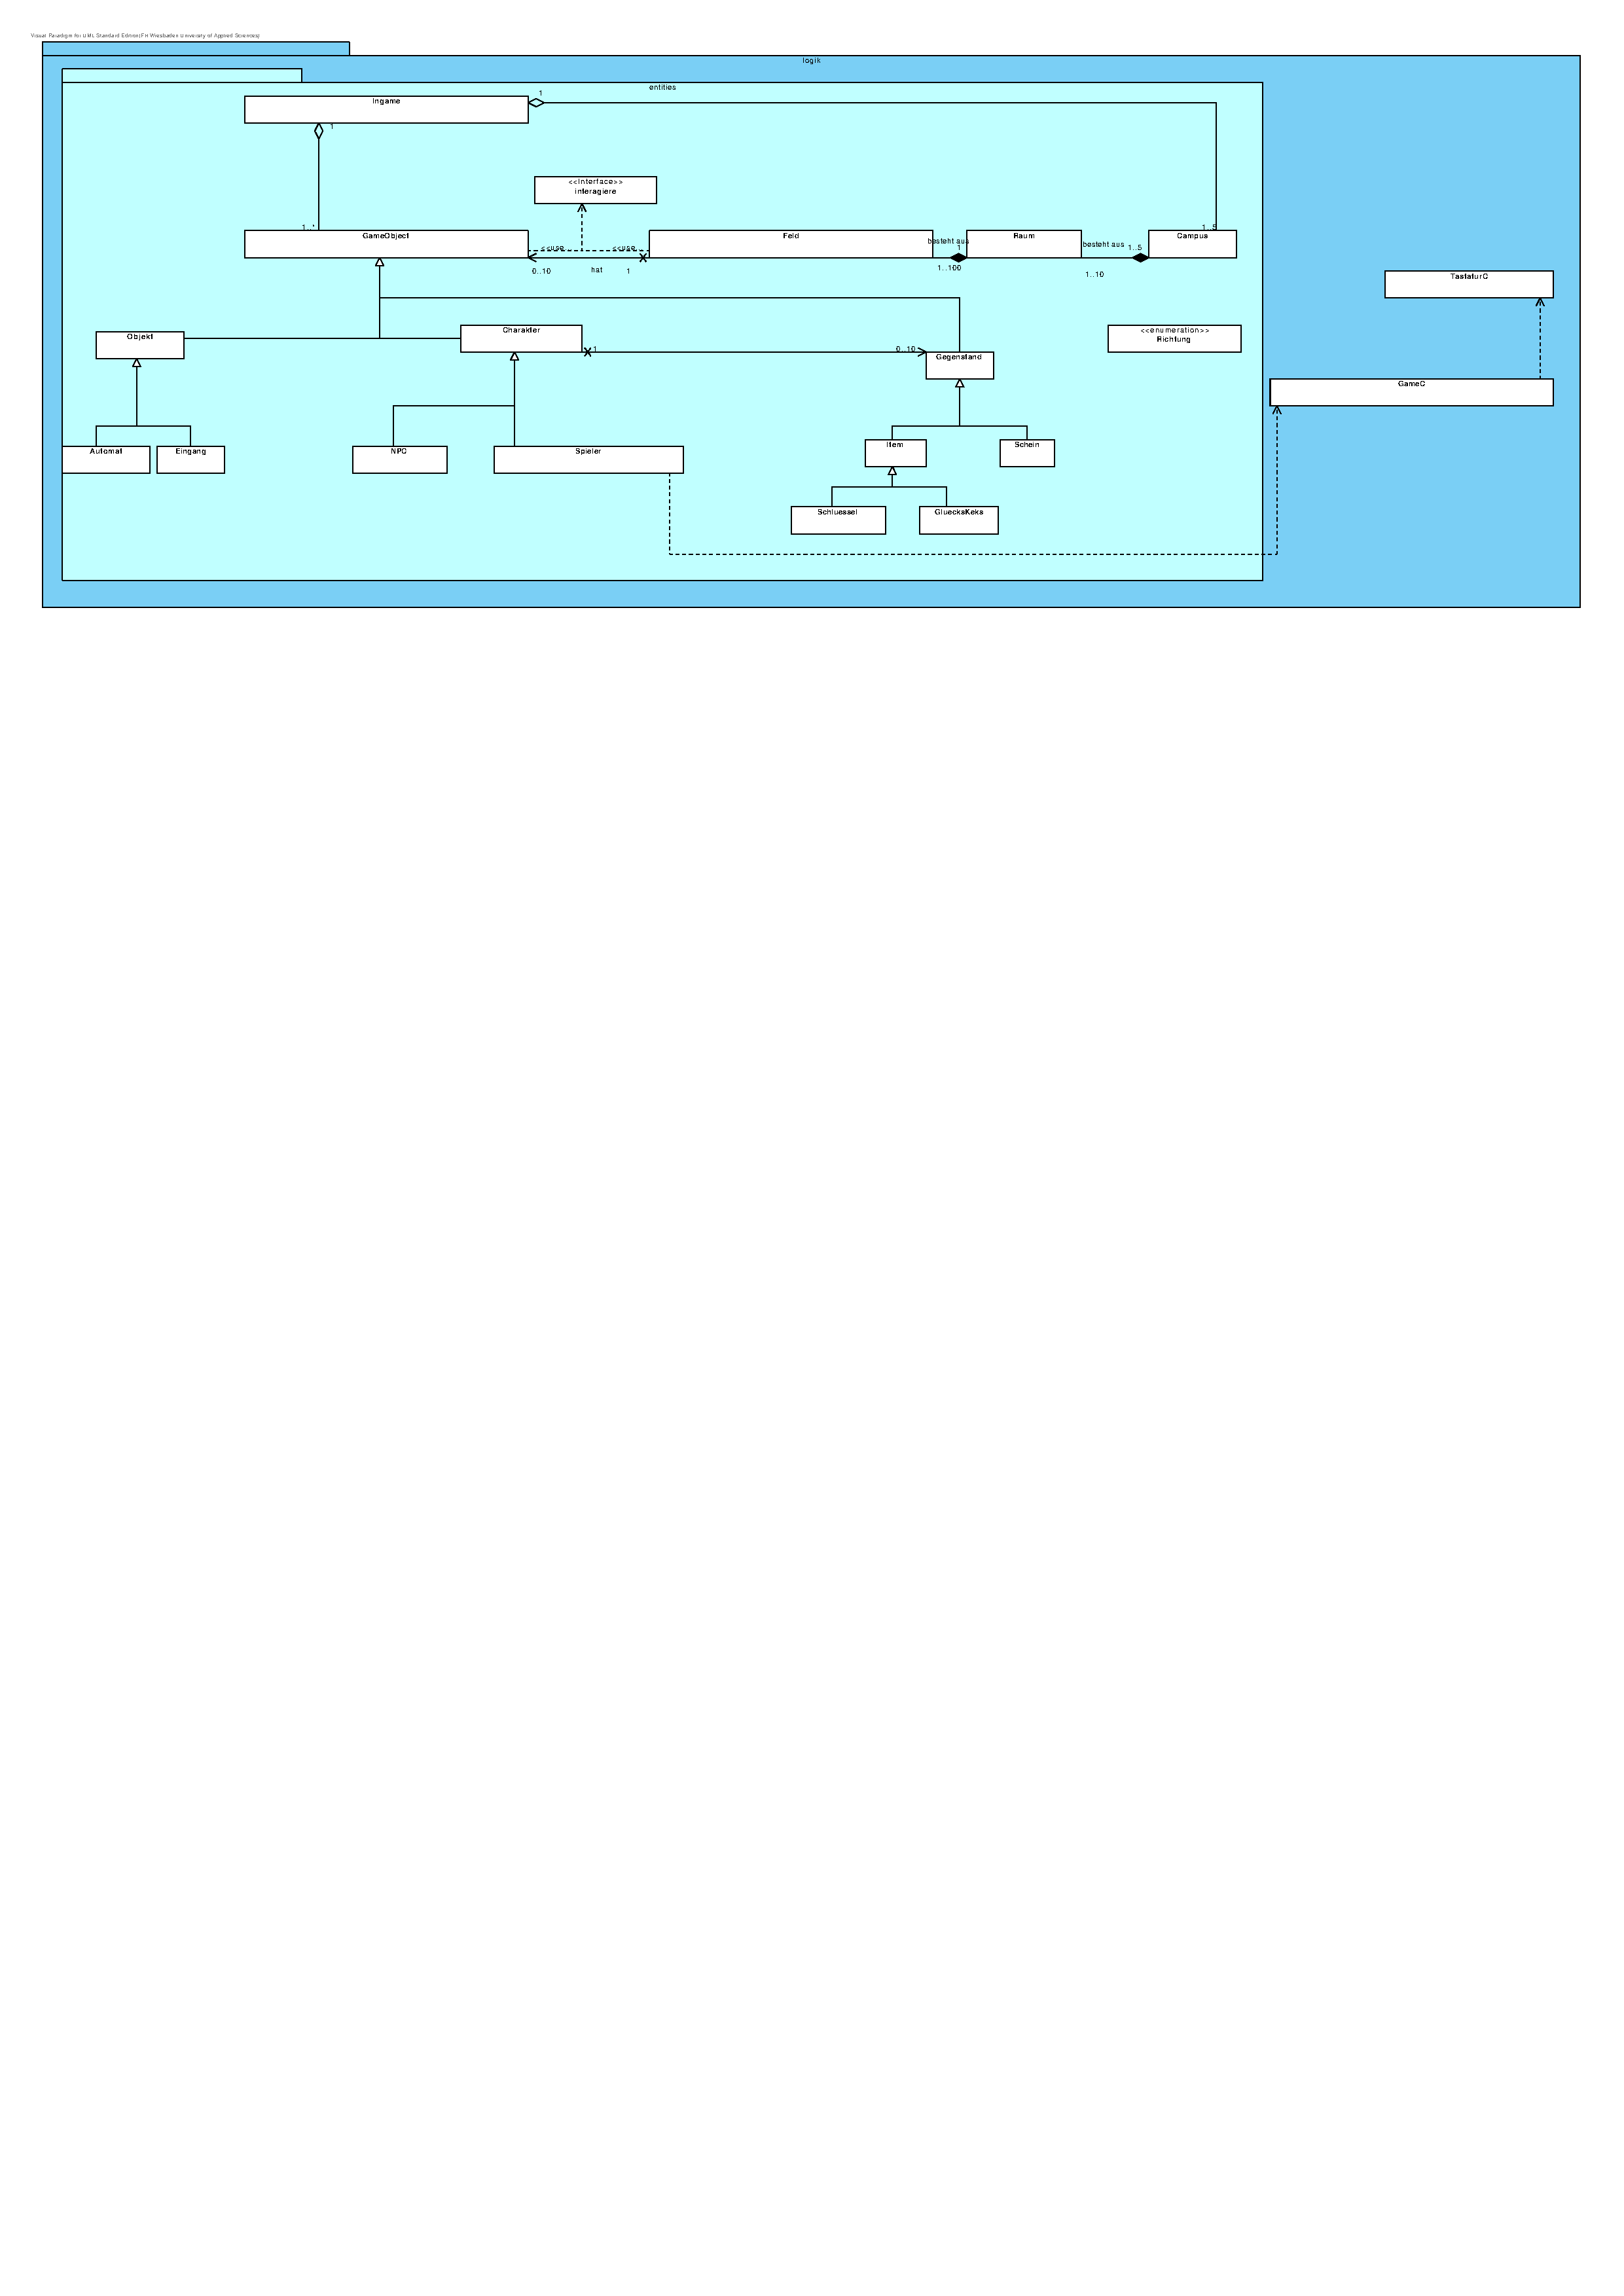
\includegraphics[trim=0cm 43cm 0cm 0cm, clip=true, width=16cm]{kapitel/bausteinsicht/logik.pdf}
	\end{center}
	\caption{Logikschicht}
	\label{fig:logik_uml}
\end{figure}

\subsection{Entities}
Das Paket \textit{entities} umfasst alle Klassen, die autark Funktionen erfüllen. Die evtl. 
benötigten Models sind im Paket \textit{models} der Datenschicht ausgelagert. Es wird hierbei das 
MVC-Pattern verwendet, um eine saubere Trennung zu gewährleisten.

\paragraph{Ingame}
Das \textit{Ingame}-Objekt beinhaltet Referenzen zu allen anderen Objekten des \textit{entities} 
Pakets. Das hat den Vorteil, dass beim Speichern nur dieses Objekt serialisiert werden muss und alle 
anderen Objekte automatisch mit gespeichert werden.

\paragraph{Feld}
Das \textit{Feld} bildet die zentrale Anlaufstelle für \textit{Spieler} und \textit{FeldV}, sodass 
es möglich ist, \glspl{Gegenstand} aufzunehmen, abzulegen und anzuzeigen. Die Kommunikation läuft 
über das Interface \textit{interagiere}.

\paragraph{Raum}
Der \gls{Raum} grenzt eine Menge von \glspl{Feld}n ein und macht sie zugänglich oder nicht. Hierdurch 
ist es beispielsweise möglich, dass der \gls{Spieler} nur \glspl{Raum} betritt, für die er einen 
Schlüssel bei sich trägt.

\paragraph{Campus}
Der \gls{Campus} umfasst alle \glspl{Raum} und grenzt die \gls{Welt} ein. Der \gls{Spieler} kann sich 
nur innerhalb eines \gls{Campus} bewegen.

\paragraph{GameObject}
Die Klasse \gls{GameObject} stellt die grundlegende Klasse für alle in der \gls{Welt} lebenden \glspl{Objekt}
dar. \glspl{GameObject} haben einen Namen und eine textuelle Beschreibung sowie ein Bild (an Stelle eines
eigenen Views).

\paragraph{Charakter}
\gls{Charakter} sind menschliche Spielfiguren, die ein eigenes \gls{Inventar} haben (also \glspl{Gegenstand}
aufnehmen können) und mit mit anderen \glspl{Charakter}n in \gls{Dialog} treten können.

\paragraph{NPC}
\gls{npcs} sind vom Computer gesteuerte \glspl{Charakter}, die zusätzlich einen \textit{Dialog} haben.
	
\paragraph{Spieler}
Die \textit{Spieler}-Klasse ist zentrales Objekt im \gls{Spiel}, denn sie stellt die virtuelle Repräsentation
des menschlichen \gls{Spieler}s dar. Jegliche Art von Interaktion wird von \gls{Spieler} (über das
\textit{interagiere}-Interface) angestoßen. Zusätzlich kann der \gls{Spieler} sich bewegen.

\paragraph{Gegenstand}
\glspl{Gegenstand} sind \glspl{Objekt} die der \gls{Spieler} aufnehmen kann. \glspl{Gegenstand} liegen z.B. auf
\glspl{Feld}n. Aber auch \glspl{Charakter} können dem \gls{Spieler} \glspl{Gegenstand} im Verlauf eines 
\gls{Dialog} überreichen. \glspl{Gegenstand} können beliebig spezialisiert sein und so zum Spielinhalt
beitragen.

\paragraph{Objekt}
Objekte sind im Gegensatz zu Gegenständen nicht aufnehmbar. Sie belegen aber einen Slot auf dem jeweiligen
Feld. Ein Beispiel für ein spezialisiertes Objekt ist der Automat, welcher bei Interaktion Gegenstand liefert.

\paragraph{Eingang}
\textit{Eingang} ist ein \textit{Objekt} und kann offen oder verschlossen sein und ist mit einem passenden
\textit{Schlüssel} aufschließbar.

\paragraph{Richtung}
Ein Enum um die \gls{Blickrichtung} des \gls{Spieler}s zu definieren. Wird z.B. von Klassen der
Darstellungsschicht verwendet, um die korrekten \glspl{Feld} im \gls{Sichtbereich} des \gls{Spieler}s
zu finden.

\subsection{Controller}
Die Controller liegen in der Logikschicht, verwenden aber kein eigenes Package. Sie kümmern sich um 
den Wechsel der Ansichten (Menu, Ingame) und um Tastatureingaben des \gls{Spieler}s.

\paragraph{TastaturC und GameC}
Zur Eingabe über die Tastatur hört \textit{TastaturC} und leitet die Eingaben an \textit{GameC} 
weiter. \textit{GameC} benachrichtigt dann, abhängig davon ob gerade ein Menu angezeigt wird oder 
nicht, die passende Klasse (\textit{Spieler} oder \textit{MenuCV}) via \textit{PropertyChangeEvent}.

\newpage

\section{Daten}
Die Datenschicht beinhaltet die Pakete \textit{models} und \textit{init}.
Hier befinden sich alle Klassen, die selbst keine direkten Spiel-Funktionen anbieten. Meist werden 
die Models durch entsprechende Factories aus Konfigurationsdateien erstellt und stehen dann Klassen 
aus der Logikschicht zur Verfügung.

\begin{figure}[h]
	\begin{center}
		%trim option's parameter order: left bottom right top , clip = true
		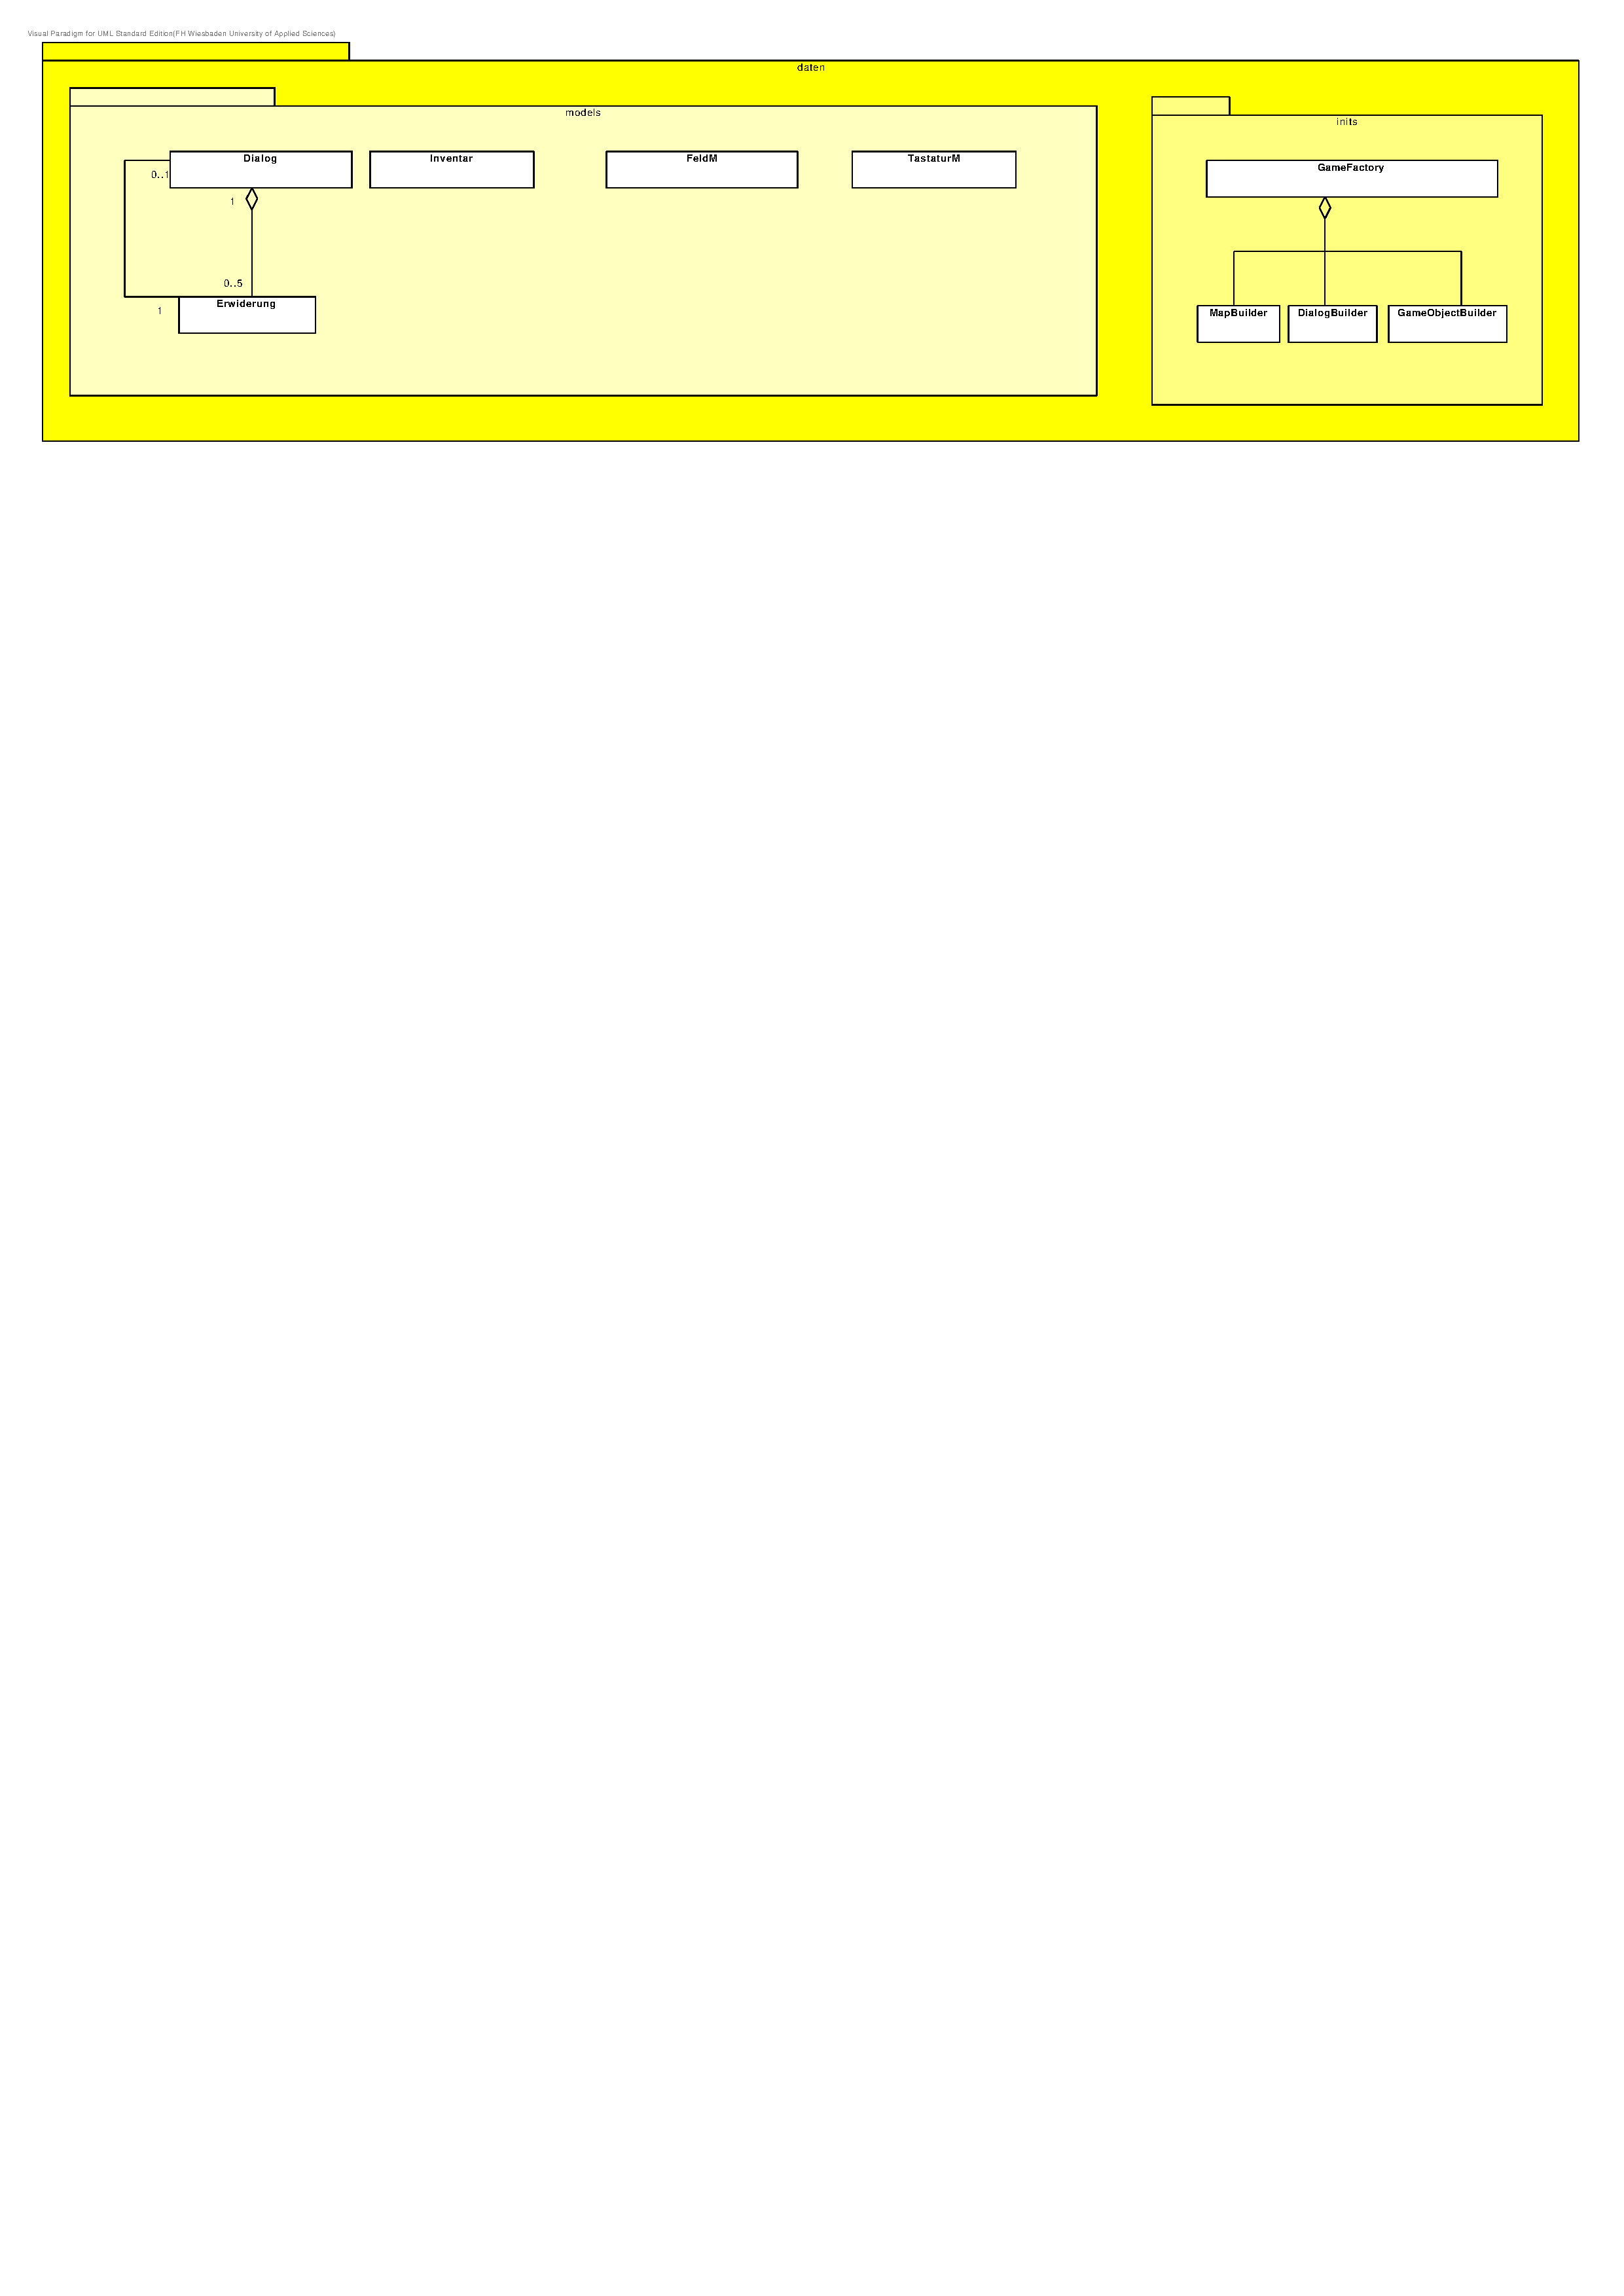
\includegraphics[trim=0cm 45cm 0cm 0cm, clip=true, width=16cm]{kapitel/bausteinsicht/daten.pdf}
	\end{center}
	\caption{Datenschicht}
	\label{fig:daten_uml}
\end{figure}

\paragraph{Dialog und Erwiderung}
Die Dialoge bilden das Rückgrat der Interaktion mit \gls{npcs}. Der Gesprächsablauf wird dabei
allerdings von Klassen in der Logikschicht übernommen. Dialoge beinhalten daher nur Referenzen zu
Erwiderungen und evtl. Geschenken, die der \gls{Spieler} erhält. Stößt der \gls{Spieler} auf einen 
\gls{Dialog}, werden ihm mögliche Erwiderungen angeboten, die er 
wählen kann. Jede Erwiderung leitet dabei auf einen neuen \gls{Dialog} oder auf das Ende der 
Unterhaltung.

\paragraph{Inventar}
Das \textit{Inventar} bietet nur rudimentäre Funktionen zum Füllen und Entnehmen von 
\glspl{Gegenstand} und wird einem \gls{Charakter} als Model mitgegeben.

\paragraph{FeldModel}
Jedes \gls{Feld} aus der Logikschicht erhält ein \textit{FeldM}, welches alle nötigen Daten aufnimmt 
und rudimentäre Funktionen (z.B. ob das \gls{Feld} begehbar ist) anbietet. Möchte der \gls{Spieler} 
einen \gls{Gegenstand} aufnehmen oder ablegen, werden diese ähnlich zu einem \gls{Inventar} im 
\textit{FeldModel} verwaltet.

\paragraph{Factories und Builder}
Die Klassen im Paket \textit{init} sind hauptsächlich Factories, die die benötigten Models aus 
Konfigurationsdateien erstellen und die passenden Models bereitstellen.

\svnid{$Id: laufzeitsicht.tex 182 2012-05-24 15:40:41Z dgens001 $}
\chapter{Laufzeitsicht}
\textit{Dieser Abschnitt stellt das Zusammenwirken der Bausteine zur Laufzeit dar.
Es wird dargelegt, wie die zuvor erarbeiteten Anforderungen erfüllt werden, wie die 
Klassen und Bausteine erzeugt, benutzt und beendet werden.}

\section{Charakterbewegung}
Wenn der \gls{Spieler} eine der Steuerungstasten 'W', 'S', 'A' und 'D' für vor- oder rückwärtige bzw.
links- oder rechtsseitige Bewegung (in dieser Reihenfolge) betätigt, wird diese Aktion von 
\textit{TastaturC} per Keyboard-Listener registriert.
Dieser feuert ein Event in Richtung des \gls{Spieler}s, der zuvor beim \textit{TastaturC} als Listener
angemeldet wurde.

Die \textit{Spieler}-Klasse wird aufgefordert ihre \textit{gehe()}-Methode aufzurufen mit der
entsprechenden \textit{Richtung} in Form eines enum-Wertes - den Himmelsrichtungen - als Funktionsparameter.
Bevor die Aktion durchgeführt werden kann, bedarf es einer Überprüfung der Zugänglichkeit des 
betroffenen Nachbarfeldes. 
Bevor die Aktion durchgeführt werden kann, bedarf es einer Überprüfung der Zugänglichkeit des 
betroffenen Nachbarfeldes. \glspl{Feld} implementieren eine \textit{begehbar()}-Methode, die 
Zugänglichkeitsinformationen für jede Richtung in einem Array verwaltet und für die angefragte 
Bewegung einen Wahrheitswert zurückliefert.

\begin{figure}[h]
	\begin{center}
		%trim option's parameter order: left bottom right top , clip = true
		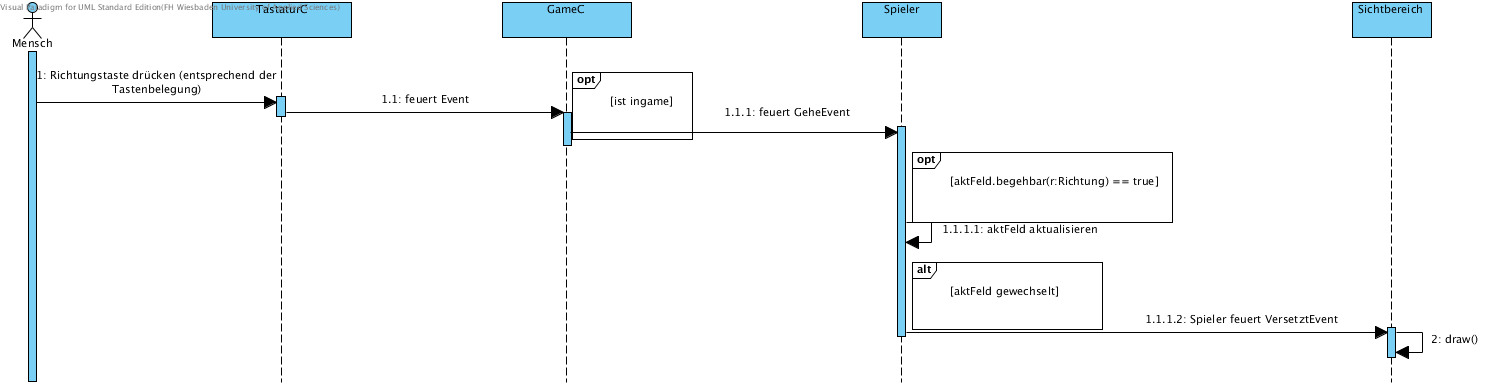
\includegraphics[trim=0cm 0cm 0cm 0cm, clip=true, width=13cm]{kapitel/laufzeitsicht/Spieler_Steuerung.png}
	\end{center}
	\caption{Charakterbewegung}
	\label{fig:steuerung_uml}
\end{figure}

Ist das \gls{Feld} zugänglich wird der \gls{Spieler} versetzt und der \gls{Sichtbereich} wird unter Verwendung der 
Darstellungsinformationen des neuen \gls{Feld}es aktualisiert.
Ist das \gls{Feld} nicht begehbar, wird eine Exception geworfen und der \gls{Spieler} wird per Textanzeige 
darüber informiert.
Auch die Tasten für das Drehen nach links und rechts - 'Q' bzw. 'E' - feuern Events, die
\textit{Spieler}-Klasse veranlassen, ihre \textit{drehe()}-Methode aufzurufen.  Auch sie erhält die gewünschte \textit{Richtung} 
als Parameter.  Das Drehen verändert die Darstellung der \glspl{Feld}, die vor dem \gls{Spieler} liegen, 
nicht aber die des \gls{Feld}es auf dem er sich aktuell befindet.

\section{Interaktion}
Betritt der \gls{Spieler} ein \gls{Feld} auf dem sich ein \gls{npc}, ein \gls{Eingang} zu einem benachbarten \gls{Raum} oder 
\gls{Gegenstand}s befinden, hat er die Möglichkeit, in letzterem Fall diese aufzunehmen bzw., in den beiden 
ersteren, mit ihnen zu interagieren.

Der \gls{Spieler} verwendet das \textit{interagiere}-Interface um mit \textit{Feld} und \textit{NPC} zu interagieren.
Dies geschieht sobald der 
\textit{TastaturC} die Betätigung der Interaktionstaste registriert. Der \gls{Spieler} bekommt zunächst, 
in textueller Form, eine Auflistung der möglichen Interaktionspartner angezeigt. Aus diesen kann 
nun per Zifferntaste einer ausgewählt werden.

\subsection{mit einem NPC}
Jeder von diesen besitzt selbst eine eigene \textit{interagiere()}, welche festlegt was passiert, 
wenn er als Interaktionspartner gewählt wird. Grundsätzlich hat jeder \textit{NPC} einen \textit{Dialog}.
Der \gls{Dialog} liegt in Form einer Baumstruktur vor, aufgebaut aus \glspl{Dialog} und \glspl{Erwiderung}.

\begin{figure}[h]
	\begin{center}
		%trim option's parameter order: left bottom right top , clip = true
		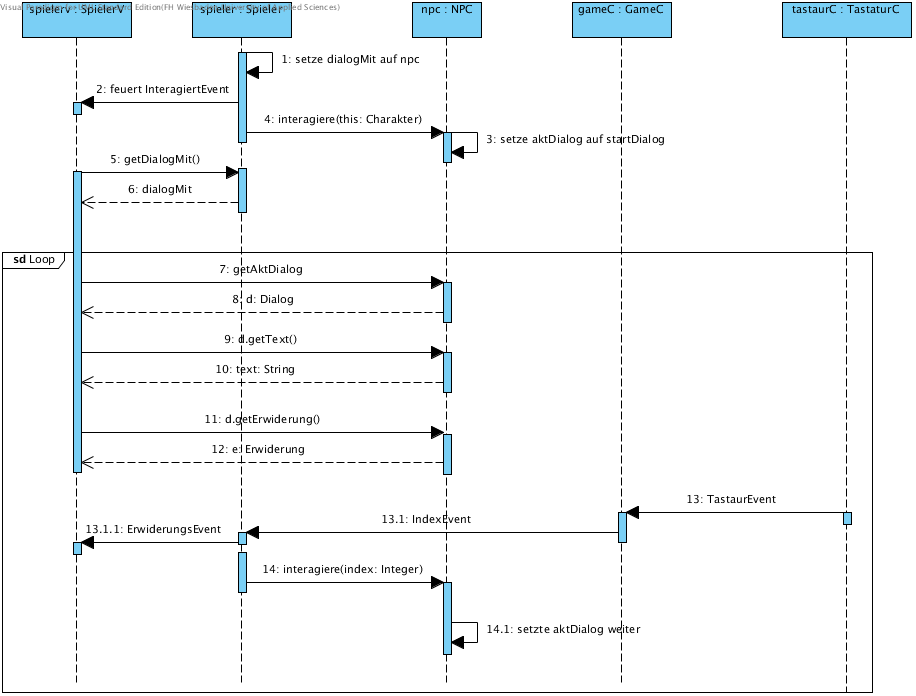
\includegraphics[trim=0cm 0cm 0cm 0cm, clip=true, width=13cm]{kapitel/laufzeitsicht/dialogMitNPC.png}
	\end{center}
	\caption{Dialog mit NPC}
	\label{fig:dialognpc_uml}
\end{figure}

Analog zur Auswahl des Interaktionspartners erfolgt die Wahl der \gls{Erwiderung} über die Zifferntasten.
Manche \gls{npcs} erwarten \glspl{Gegenstand} vom \gls{Spieler}. Im Laufe des \gls{Dialog}es würde an einem festgelegten 
Knoten des Baumes überprüft, ob der entsprechende \gls{Gegenstand} im Handslot des \gls{Spieler}s vorhanden ist.
Ausgehend vom Ergebnis dieser Überprüfung, wird entlang des entsprechenden Astes weiter durch die 
Baumstruktur navigiert.

In der Basisversion der Anwendung ist vorgesehen, dass der \gls{Spieler} die \textit{interagiere()}-Methode des \gls{npcs} 
mit sich selbst als Funktionsparameter aufruft. Hiermit wird ihm signalisiert, dass ein \gls{Dialog} 
gestartet werden soll. Für Erweiterungen sind alternative Interaktionsmöglichkeiten denkbar, 
ausgelöst durch Übergabe weiterer Parameter, wie beispielsweise einer Waffe im Handslot des \gls{Spieler}s.

\newpage

\subsection{mit einem Objekt}
Ein unverschlossener \gls{Eingang}, dessen \textit{interagiere()}-Methode aufgerufen wird, öffnet sich und gibt den 
dahinterliegenden Weg frei.
Ist er aber verschlossen, würde der \gls{Eingang}, ähnlich wie der \gls{npc}, einen \gls{Gegenstand} erwarten. 
Sinnvollerweise eine Art von \textit{Schluessel}, je nach Öffnungsmechanismus. Das matchen von \textit{Schluessel} und 
\textit{Eingang} geschieht anhand ihrer Nummer.

\subsection{mit einem Gegenstand}
In diesem Fall findet keine Interaktion wie in den ersten beiden Fällen statt. Will der \gls{Spieler} einen 
\gls{Gegenstand} vom \textit{Feld} aufnehmen, auf dem er sich aktuell befindet, geschieht das durch das \textit{interagieren}-Interface.

\begin{figure}[h]
	\begin{center}
		%trim option's parameter order: left bottom right top , clip = true
		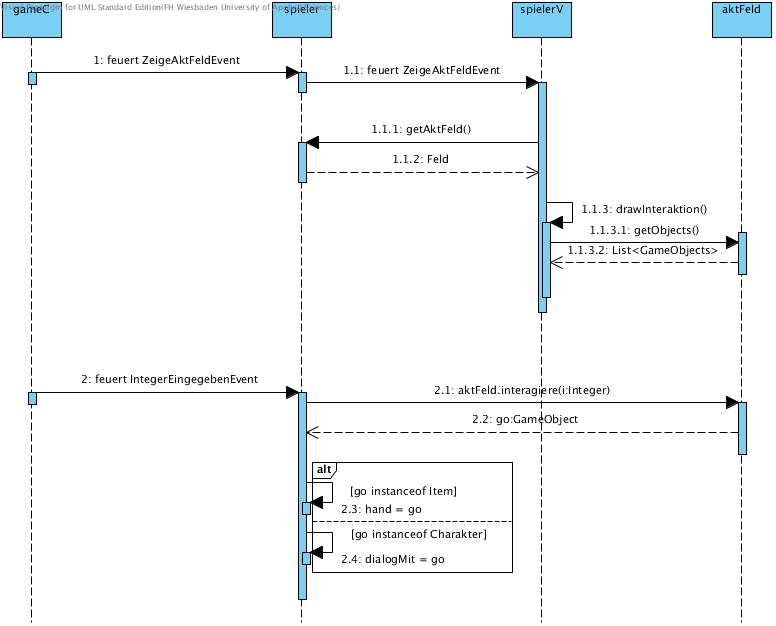
\includegraphics[trim=0cm 0cm 0cm 0cm, clip=true, width=13cm]{kapitel/laufzeitsicht/itemAufnehmen.png}
	\end{center}
	\caption{Gegenstand aufnehmen}
	\label{fig:item_uml}
\end{figure}

Die Referenz im \textit{FeldM} auf das entsprechenden \gls{Gegenstand} wird gelöscht
und eine neue auf den Handslot des \gls{Spieler}s hergestellt. Dieser muss zum Aufnehmen eines neuen \gls{Gegenstand}s 
frei sein. Ist er es nicht, kommt es zur Exception. 
Für spätere Versionen der Anwendung ist es denkbar einen zweiten Handslot einzuführen, der es dann
erlaubt, zwei in den Händen befindliche \glspl{Gegenstand} über ihre \textit{interagiere()}-Methode zu kombinieren.

\subsection{mit dem Inventar}
Möchte der Spieler ein Item aus seinem Handslot in sein Inventar ablegen, geschieht dies ähnlich wie
bei der Übergabe eines Items vom Feld an den Handslot. Die Referenz zwischen Handslot und Item wird 
entfernt, während zwischen Inventar und Item eine neue geschaffen wird.
Soll ein Item aus dem Inventar in den Handslot genommen werden, erhält der Spieler beim Betätigen 
der \textit{inDieHand}-Taste, wieder in textueller Form, eine Auswahl der Gegenstände, die sich in seinem 
Inventar befinden. Per Zifferntaste kann ausgewählt werden. Die Referenzen werden entsprechend 
aufgelöst. Analog zum Feld, stellt das Inventar sowohl eine nehmen-, als auch eine \textit{geben}-Methode 
zur Verfügung.

\begin{figure}[h]
	\begin{center}
		%trim option's parameter order: left bottom right top , clip = true
		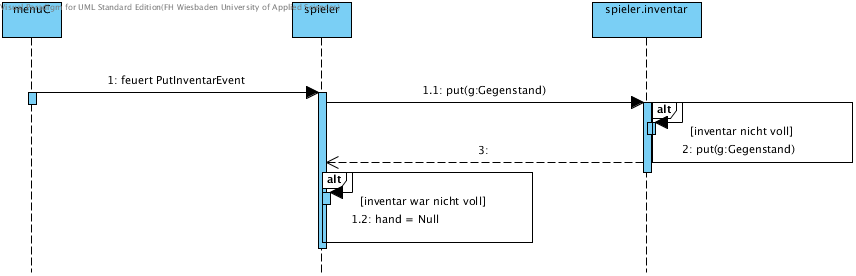
\includegraphics[trim=0cm 0cm 0cm 0cm, clip=true, width=13cm]{kapitel/laufzeitsicht/itemHandInventar.png}
	\end{center}
	\caption{Item ins Inventar}
	\label{fig:inventar_uml}
\end{figure}

\subsection{Neues Spiel}
Der Spieler befindet sich nach dem Spielstart im Hauptmenü. Hier steht ihm die Option Neues Spiel zur 
Verfügung. Startet der Spieler ein neues Spiel ruft dies die \textit{neuesSpiel()}-Methode in \textit{GameC} auf. 
Diese startet die \textit{getGameInstance()}-Methode in der \textit{GameFactory}. Dadurch werden der 
\textit{MapBuilder}, \textit{DialogBuilder} und der \textit{GameObjectBuilder} ausgeführt, welche ein spielbares 
\textit{Ingame} (Spiel) initialisieren. Der \textit{GameC}prüft darauf hin ob ein \textit{Ingame}-Objekt vorhanden 
ist und setzt das Attribut \textit{ingame}(Boolean) entsprechend auf "true". 
Ist der Boolean \textit{ingame} auf true, wird ein Event gefeuert das die \textit{drawIngame()}-Methode der 
\textit{Fenster}-Klasse innerhalb der Darstellungsebene aufruft. Durch \textit{drawIngame()} wird dann die Ansicht 
des Spiels gezeichnet. Zudem startet der \textit{GameC} das Spiel(Gameloop).

\begin{figure}[h]
	\begin{center}
		%trim option's parameter order: left bottom right top , clip = true
		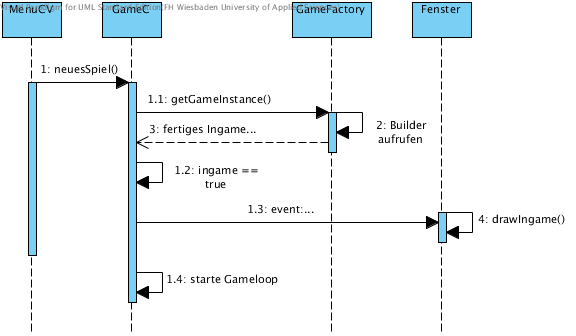
\includegraphics[trim=0cm 0cm 0cm 0cm, clip=true, height=7cm]{kapitel/laufzeitsicht/neuesSpiel.png}
	\end{center}
	\caption{neues Spiel}
	\label{fig:nspiel_uml}
\end{figure}

\newpage

\subsection{Spiel speichern}
Möchte der Spieler seinen aktuellen Spielstand speichern, gelangt er über die entsprechende Taste in das
Pausemenü. Hier findet er den Spiel speichern-Button. Der Spiel speichern-Button löst nach dem betätigen die 
\textit{spielSpeichern()}-Methode des \textit{GameC} aus. Da dieser das Objekt \textit{Ingame} besitzt, kann er die 
\textit{serialisieren()}-Methode der \textit{Ingame}-Klasse aufrufen. Diese speichert alle aktuellen Spieldaten als 
Savegame auf der Festplatte.

\begin{figure}[h]
	\begin{center}
		%trim option's parameter order: left bottom right top , clip = true
		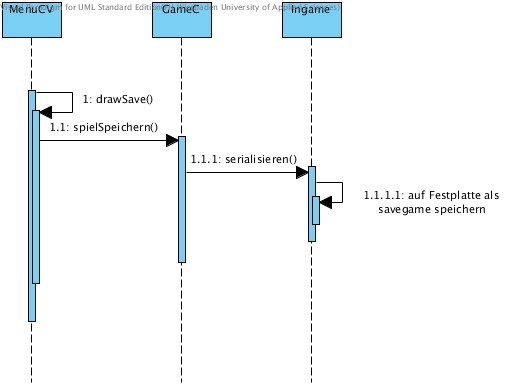
\includegraphics[trim=0cm 0cm 0cm 0cm, clip=true, width=13cm]{kapitel/laufzeitsicht/spiel_speichern.jpg}
	\end{center}
	\caption{Spiel speichern}
	\label{fig:speichern_uml}
\end{figure}
\newpage
\subsection{Spiel laden}
Über das Pausemenü, während einer Spielunterbrechung, oder das Hauptmenü nach dem Spielstart kann der Spieler 
einen Spielstand laden. Wenn ein Spiel geladen werden soll, wird zunächst über die \textit{drawLoad()}-methode des 
\textit{MenuCV} das entsprechende Fenster zur Auswahl eines Savegames gezeichnet. Wurde ein Spielstand gewählt,
wird die \textit{spielLaden()}-Methode zusammen mit dem Savegame als Parameter im \textit{GameC} aufgerufen. 
Der \textit{GameC} startet die \textit{getGameInstanceFromSavegame()}-methode der \textit{GameFactory}, welche das 
übergebene Savegame deserialisiert und ein fertiges \textit{Ingame}-Objekt erstellt. Der \textit{GameC} prüft 
daraufhin ob ein solches spielbares \textit{Ingame}-Objekt vorhanden ist und gibt dann den Boolean \textit{ingame}(true) 
zurück. Ist \textit{ingame} auf true gesetzt feuert der \textit{PropertyChangeListener} ein Event an die 
\textit{Fenster}-Klasse in der Darstellungsebene. Diese zeichnet über die \textit{drawIngame}-Methode das sichtbare Spiel
anhand der des \textit{Ingame}-Objekts, dass aus den Savegamedaten entstanden ist. Zudem startet der \textit{GameC} 
das Spiel.
\\

\begin{figure}[h]
	\begin{center}
		%trim option's parameter order: left bottom right top , clip = true
		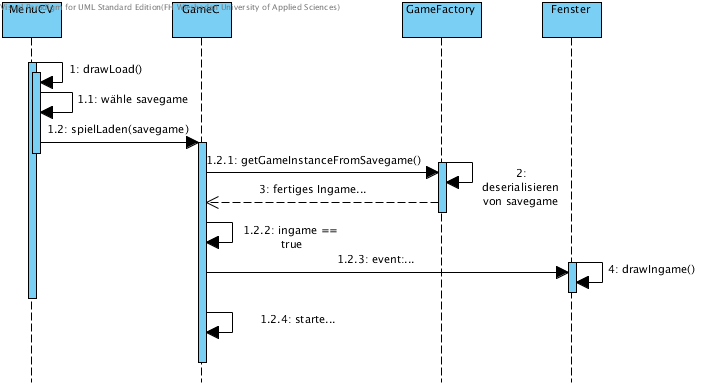
\includegraphics[trim=0cm 0cm 0cm 0cm, clip=true, width=13cm]{kapitel/laufzeitsicht/spielLaden.png}
	\end{center}
	\caption{Spiel laden}
	\label{fig:laden_uml}
\end{figure}

\svnid{$Id: musterundkonzepte.tex 180 2012-05-24 15:26:04Z dgens001 $}
\chapter{Muster und Konzepte}

\subsection{Listener-Konzept}
Die Anwendung verwendet \textit{PropertyChangeListener} und \textit{PropertyChangeSupport}.
Erstere werden von solchen Klassen verwendet, deren Objekte auf Ereignisse aus anderen Bereichen des \gls{Spiel}s warten.
Sie melden sich als Listener für bestimmte Attribute und Funktionen an. Ändern sich diese, erfahren die Listener
das und können im eigenen Objekt für Methodenaufrufe sorgen.
 
Für das Erfahren dieser Änderungen ist der \textit{PropertyChangeSupport} zuständig. 
Aus der Klasse heraus, in der er sich befindet, \textit{feuert} er \textit{PropertyChangeEvents}, 
die an die zugehörigen \textit{PropertyChangeListener} adressiert sind.

\subsection{MVC}
Für die Darstellung der Anwendung ist die Klasse \textit{Fenster} verantwortlich, unabhängig davon in welchem Modus 
- Menü oder Ingame - sich das \gls{Spiel} im Momemt befindet. Sie setzt sich wiederum aus verschiedenen Klassen, 
den Views, zusammen. Diese vereinen in sich jeweils die Informationen, die für die Darstellung der entsprechenden 
View von Nöten sind.

Die \textit{SpielerV} ist für die Anzeige des \gls{Statusbereich}s verantwortlich. Ihre Informationen kommen zum einen vom
\textit{Spieler} selbst und andererseits von \textit{NPC}s, \textit{Objekt}en oder \textit{Feld}ern mit denen aktuell interagiert wird.
\textit{Spieler} feuert Events, die den View anweist, die benötigten Informationen aus den entsprechenden Models zu lesen.
 
Beispiele für die Darstellung durch die \textit{SpielerV} sind \glspl{Dialog} und das Aufnehmen von \glspl{Item} von 
einem \textit{Feld} in die \textit{Hand} von \textit{Spieler}.

Bei der Klasse \textit{Sichtbereich} handelt es sich um die \gls{Welt} aus der Ego-Perspektive des \gls{Spieler}s.
Der gesamte \textit{Sichtbereich} setzt sich aus 32 \textit{JPanel}s zusammen, durch die sichergestellt wird, dass jede in der
Anwendung vorgesehene Kombination von Texturen darstellbar ist.

Es lassen sich zwei Unterbereiche abgrenzen. Das \textit{Feld} auf dem sich der \gls{Spieler} aktuell befindet und die beiden
in \gls{Blickrichtung} vor ihm liegenden \glspl{Feld} werden samt darauf befindlicher \glspl{Gegenstand} und \gls{npcs} dargestellt.
Alle anderen \glspl{Feld} und zugehörige Wände werden ausschließlich als Texturen angezeigt.

Unabhängig davon werden alle \glspl{Feld} einzeln durch eine separate \textit{FeldV} erstellt. Die Informationen hierzu 
kommen wiederum von den Models der einzelnen Felder(\textit{FeldM}).

Die letzte verbleibende View ist die \textit{MenuCV}, die gleichzeitig als Controller fungiert. 
Da das Menü nur eine grafische Oberfläche ohne abgrenzbare Logik ist, ist diese Zusammenführung sinnvoll.
Das Menü wird vor dem Start eines neuen oder Laden eines bereits begonennen \gls{Spiel}s als Hauptmenü angezeigt. 
Es dient gleichzeitig als Pausemenü, sollte das \gls{Spiel} zwischendurch unterbrochen werden.
In diesem Fall behalten die oben genannten Views ihre aktuellen Informationen, werden aber nicht angezeigt während
das Menü aktiv ist.

Die einzelnen Views erben jeweils von der Klasse \textit{JPanel}. Die Klasse \textit{Fenster}, die, wie oben erklärt die 
Views zur gesamten \gls{Anzeige} zusammensetzt, erbt von der Klasse \textit{JFrame}.
Die Views und das \textit{Fenster} implementieren Funktionen des o.g. Listener-Konzeptes, um ihre
Darstellungs-Informationen von den entsprechenden Models zu erhalten.


%\svnid{$Id: entwurfsentscheidungen.tex 180 2012-05-24 15:26:04Z dgens001 $}
\chapter{Entwurfsentscheidungen}


% ---------------------------------- Anhänge -----------------------------------
% In diesem Teil werden alle Anhänge eingefügt, die auch als ganz normale Kapi-
% tel abgelegt werden.
%\appendix
%\include{kapitel/anhang}

% Ausgabe des Glossars (oder der Glossare, wenn mehrere definiert sind)
%\glsaddall
\printglossary
\end{document}
